\chapter{Window Fourier Transform} 
\begin{figure}[ht]
    \centering
    \incfig{wftonf}
    \caption{WFT of $f$}
    \label{fig:wftonf}
\end{figure}

\begin{defn}[Window]
    Let $ w $ a window such that $ w \in \mathscr{L}^2 \wedge \mathscr{L}^2 $ and $ \left
    | \widehat{w} \right |  $ is an odd function and $ \| w \|^{ }_{ 2} = 1 $
    We define 
    \[
        w _{ \lambda, b }^{  } (t) = w(t-b) e^{ 2i\pi\lambda t} 
    \]
    then $ \forall f \in \mathscr{L}^2(\mathbb{R})   $ the WFT is defined as 
    \[
        W_f(\lambda,b) = \int\limits_{-\infty}^{\infty} f(t) \overline{w}_{\lambda, b}(t)
        \ dt 
    \]
    \label{def:Window}
\end{defn}

Some properties 
\begin{enumerate}[label={(\alph*)}]
    \item Conservation of Energy : 
        \[
            \int\limits_{-\infty}^{\infty} \left | f(t)  \right | ^2 \ dt =
            \int\limits_{-\infty}^{\infty} \int\limits_{-\infty}^{\infty} \left |
            W_f\left( \lambda, b\right)  \right | ^2 \ d\lambda \ db
        \]
    \item Reconstruction formula : 
        \[
            f(x) = \int\limits_{-\infty}^{\infty} \int\limits_{-\infty}^{\infty}
            W_f(\lambda, b) w_{\lambda, b} (t) \ d\lambda \ db
        \]
\end{enumerate}
\subsubsection{Comment:}
How to choose $ w $? In practice $ w $ is centered and symmetric on 0. We want $
w_{\lambda, b}(t) $ centered on $ \left( \lambda, b\right)  $. 
\section{Exercises : Atoms}
\label{sec:Exercises : Atoms}
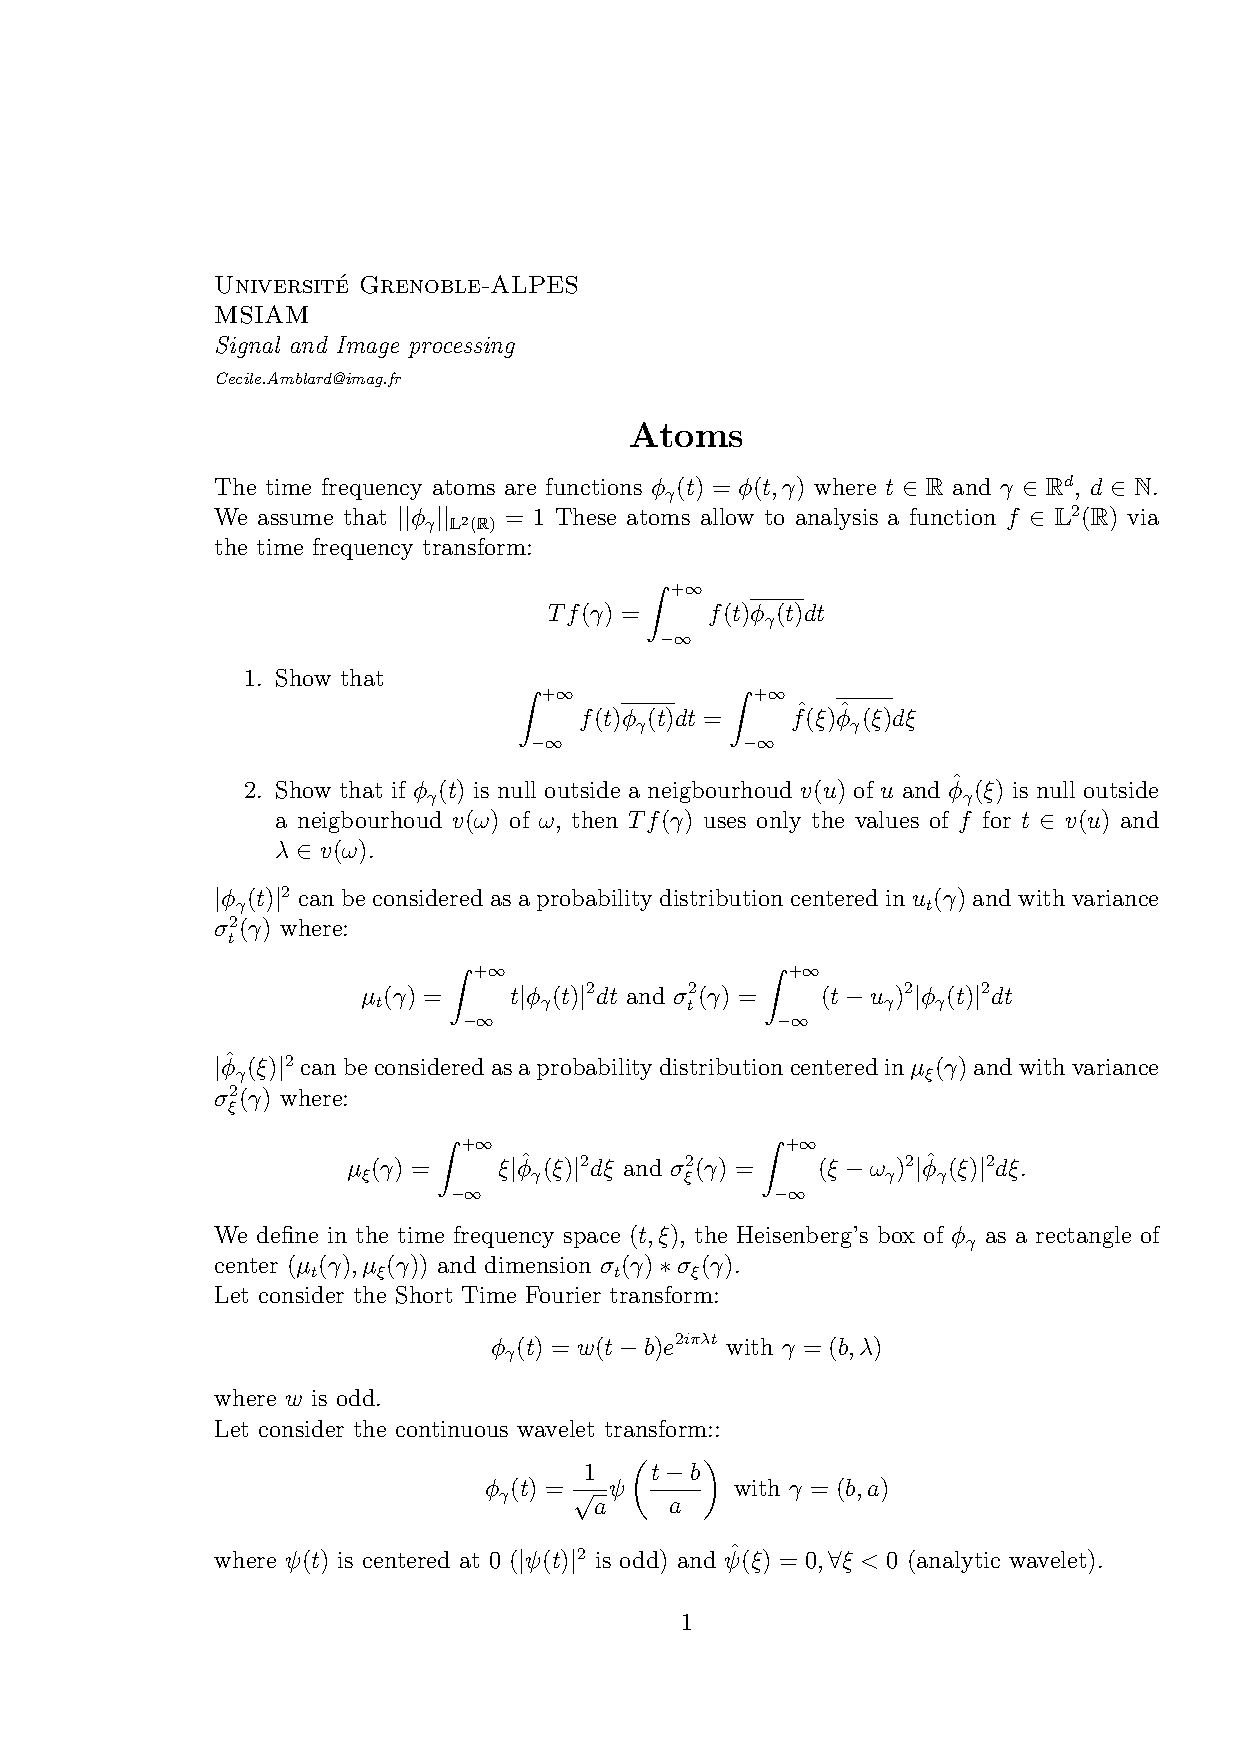
\includepdf[pages=-]{References/TDTempsFreq.pdf} 
\subsubsection{Part 1)}


\subsubsection{Part 2)}
\begin{align*}
    \mu_t(\gamma) &= \int\limits_{-\infty}^{\infty} t \left | \phi_{\gamma}(t) \right | ^2
    \ dt \\
                  &= \int\limits_{-\infty}^{\infty} t \left | w(t-b) e^{ 2i\pi\lambda t}  \right | ^2
    \ dt \\
                  &= \int\limits_{-\infty}^{\infty} (u+b) \left | w(u)\right | ^2\ du \\
                   &= b \text{ since } \| w \|^{ }_{ 2} = 1; \| w \|^{ 2}_{ } \text{ is
                   even }
\end{align*}

\begin{align*}
    \sigma_t^2 &= \int\limits_{-\infty}^{\infty}\left( t-\mu_t\right) ^2 \left |
    \phi_{\gamma} (t) \right | ^2 \ dt \\ 
 &= \int\limits_{-\infty}^{\infty} \left( t-b\right) ^2 \left | w\left( t-b\right)  \right
 | ^2 \ dt \\ 
 &= \int\limits_{-\infty}^{\infty} u^2 \left | w(u) \right | ^2 \ du \\ 
  &= \sigma^2_w \\ 
\end{align*}

\begin{align*}
    \widehat{\phi}(\xi) &= \int\limits_{-\infty}^{\infty} \phi_{\gamma}(t) e^{ -2i\pi\xi t}
    \ dt \\
     &= \int\limits_{-\infty}^{\infty} w(t-b) e^{ -2i\pi t(\xi - \lambda) } \ dt \\
     &= \int\limits_{-\infty}^{\infty} w(u) e^{ -2i\pi(u+b)(\xi-\lambda)} \ du \\
     &= e^{ 2i\pib(\lambda-\xi)} \int\limits_{-\infty}^{\infty} w(u) e^{ -2i\pi u (\xi -
     \lambda) } \ du  \\
     &= e^{ 2i\pi b (\lambda - \xi) } \widehat{w}(\xi - \lambda)
\end{align*}
and we have that 
\begin{align*}
    \left | \phi_{\gamma}(\xi) \right |  &= \left | \widehat{w}\left( \xi - \lambda\right)
    \right |\ d\xi   \\ 
    \mu_{\xi}  &= \int\limits_{-\infty}^{\infty}  \xi \left | \widehat{w}\left( \xi -
    \lambda\right)  \right |^2 \ d\xi  \\ 
               &= \int\limits_{-\infty}^{\infty} \left( f + \lambda \right) \left |
               \widehat{w}(f) \right | ^2 \ df \\ 
                &= \lambda  \\ 
\end{align*}
Finally, this all implies that 
$ \sigma _{ \xi }^{ 2 }  = \int\limits_{-\infty}^{\infty} f^2 \left | \widehat{w}(f)
\right | ^2 \ df = \sigma _{ \widehat{w}  }^{ 2 } $. 
$ \\ $
$ w_{\gamma}  $ is a signal whose energy can be represented by a box, like
\ref{fig:heisunbox}, if $ \gamma  $ changes, the center of the box changes but the
dimension of the box does not change. Atoms $ \phi_{\gamma}  $ are represented by temporal
spatial boxes of the same size. If the lengths of support of $ \phi_{\gamma}  $ is not
large enough, we can't capture low frequency. If the length of the support is too large,
we analyze high frequency component of the signal but lose time accuracy.

\chapter{Continuous Wavelet Transform} 
\subsubsection{Motivations}
We want to analyze a signal through atoms whose dimensions changes versus frequencies. 
\begin{defn}[Analyzing function]
    The continuous wavelet transform uses an analyzing function
    \[
        \psi_{a,b}(t) = \frac{ 1 }{ \sqrt{a}  } \psi \left( \frac{ t-b }{ a } \right) 
    \]
    where b is the translation parameter and a is the scale parameter. 
    \label{def:Analyzing function}
\end{defn}
For each $ \psi  $ there exists an exact link between scale and frequency. 
\begin{figure}[ht]
    \centering
    \incfig{psinormal}
    \caption{$\psi_{[1,0]}$ }
    \label{fig:psinormal}
\end{figure}

\begin{figure}[ht]
    \centering
    \incfig{psistretch}
    \caption{Dilation}
    \label{fig:psistretch}
\end{figure}

\begin{figure}[ht]
    \centering
    \incfig{contraction}
    \caption{contraction}
    \label{fig:contraction}
\end{figure}
\newpage
High scale captures low frequencies, and low scale saptures hight frequency. 

$ \\ $
\newpage
\begin{defn}[Wavelet]
    Let $ \psi \in \mathscr{L}^1(\mathbb{R}) \cap \mathscr{L}^2(\mathbb{R})   $ such that 
    \begin{enumerate}
        \item \[
                \int\limits_{-\infty}^{\infty} \frac{ \left | \widehat{\psi}(\lambda)
                \right | ^2}{ \left | \lambda  \right | }\ d\lambda = K < \infty
        \]
    \item $ \| \psi \|^{ }_{ 2} = 1 $. 
    \end{enumerate}
    Let 
    \[
        \psi_{a,b}(t) = \frac{ 1 }{ \sqrt{a}  } \psi \left( \frac{ t-b }{ a } \right) 
    \] and $ \forall f \in \mathscr{L}^2(\mathbb{R})$ we consider the coefficients of an
    ondelette to be given by 
    \[
        C_f(a,b) = \int\limits_{-\infty}^{\infty} f(t) \overline{\psi}_{a,b}(t) \ dt
    \]
    \label{def:Wavelet}
\end{defn}

We have the following properties. 
\begin{enumerate}[label={(\alph*)}]
    \item Conservation of Energy : 
        \[
        \frac{ 1 }{ K } \int\limits_{-\infty}^{\infty} \int\limits_{-\infty}^{\infty}
        \left | C_f(a,b)  \right | ^2 \frac{ dadb }{ a^2  }
        \]
    \item Reconstruction Formula : 
        \[
            \frac{ 1 }{ K } \int\limits_{-\infty}^{\infty} \int\limits_{-\infty}^{\infty}
            C_f(a,b) \psi_{a,b} (x) \frac{ dadb }{ a^2 } 
        \]
\end{enumerate}
In practice we choose $ \psi $ such that $ \widehat{\psi}(0) = 0 $ oscilating function. 

Give the formulas and graphs for Haar wavelet, Mexican Hat, and Morlet wavelet. 

\subsection{Problem #?}
\label{subsec:Problem #?}
\begin{align*}
    \psi_{a,b} &= \frac{ 1 }{ \sqrt{a}  } \psi\left( \frac{ t-b }{ a } \right) 
\end{align*}
\begin{align*}
    \mu_t(\gamma)  &= \int\limits_{-\infty}^{\infty} t \left | \phi_{\gamma} (t) \right |
    ^2 \ dt \\ 
     &= \int\limits_{-\infty}^{\infty} t \left | \frac{ 1 }{ \sqrt{a}  } \psi\left( \frac{ t-b }{ a } \right)\right |^2 \ dt \\  
      &u = \frac{ t-b }{ a }  \implies t = au+b \text{ and } dt = a \ du\\ 
      \mu_t &= \frac{ 1 }{ a } \int\limits_{-\infty}^{\infty} \left( au+b\right) \left |
      \psi_{a,b} (u)  \right | ^2 \ adu  \\
       &= b \text{ since } \psi \text{ even and  } \| \psi  \|^{ 2}_{ 2} = 1 \\ 
\end{align*}

\begin{align*}
    \sigma_t^2 &= \frac{ 1 }{ a } \int\limits_{-\infty}^{\infty} \left( t-b\right) ^2 \left
    | \psi \left( \frac{ t-b }{ a } \right)  \right | ^2 \ dt \\ 
     &= \int\limits_{-\infty}^{\infty} a^2 u^2 \left | \psi\left( u\right)  \right | ^2 \
     du \\ 
      &= a^2\sigma_4^2 \\ 
\end{align*}

\begin{align*}
    \widehat{\psi}_{a,b} (\lambda)   &= \frac{ 1 }{ \sqrt{a}  }
    \int\limits_{-\infty}^{\infty} \psi \left( \frac{ t-b }{ a }\right)   e^{
    -2i\pi\lambda t} \ dt  \\ 
                                     &= \sqrt{a} 
    \int\limits_{-\infty}^{\infty} \psi \left( u \right)   e^{
    -2i\pi\lambda[au+b] } \ dt  \\ 
                                     &= \sqrt{a} e^{ -2i\pi\lambda b} \psi(a\lambda)  \\ 
\end{align*}

\begin{align*}
    \mu_{\xi}(\gamma) &= \int\limits_{-\infty}^{\infty} \lambda a \left |
    \widehat{\psi}\left( a\lambda\right)  \right | ^2 \ d\lambda \\ 
                      &= \int\limits_{-\infty}^{\infty} f \left | \widehat{\psi} (f)
                      \right | ^2 \frac{ df }{ a }  \\ 
                       &= \frac{ 1 }{ a } \int\limits_{-\infty}^{\infty} f \left |
                       \widehat{\psi} (f)  \right | ^2 \ df  \\ 
                        &= \frac{ ?  }{ a }  \\ 
\end{align*}
Where $ ?   $ is maybe $ \Gamma $
The previous calculation shows that frequency is the inverse of scale. 

\begin{align*}
    \sigma _{ \xi }^{ 2 } (\gamma)  &= \int\limits_{-\infty}^{\infty} \left( \lambda -
    \frac{ \Gamma  }{ a } \right) a \left | \widehat{\psi} (a\lambda)  \right | ^2 \
    d\lambda  \\ 
     &= \int\limits_{-\infty}^{\infty} \left( \frac{ f - \Gamma }{ a } \right) ^2 \left |
     \widehat{\psi} (f)\right | ^2 \ df   \\ 
      &= \frac{ 1 }{ a^2 } \int\limits_{-\infty}^{\infty} \left( f - \Gamma\right) ^2
      \left | \widehat{\psi}(f) \right | ^2 \ df = \frac{ 1 }{ a^2  } \sigma _{
      \widehat{\psi} }^{ 2 }  \\ 
\end{align*}





\section{Random Discussion}
\label{sec:Random Discussion}
We have that
\[
\int\limits_{ }^{ } \left | f(t)  \right | ^2 \ dt  
\]
gives us the energy density which we can think of as a probability density. 
Think about the frequency space 

In Window Fourier transform, the dimension of boxes are independent of position $ \left( \mu_t,
\mu_\xi \right)  $ of the 

In continuous wavelet transform 
dimension of $ \sigma  $ on the scale $ a $. 

The aim of CWT is to analyze non-stationary signals that have height variations with less
regularity. 
